\documentclass{beamer}

\mode<presentation> { \usetheme{gruvbox} }
\setbeamerfont{frametitle}{size=\huge}


\usepackage{graphicx} % Allows including images
\usepackage{booktabs} % Allows the use of \toprule, \midrule and \bottomrule in tables
%\usepackage{listings}             % Include the listings-package
\usepackage{minted}
\usepackage{tikz}
\usepackage{drawstack}
\usetikzlibrary{calc,shapes.callouts,shapes.arrows,chains,positioning,fit,shapes, arrows.meta, arrows}
\usepackage{verbatimbox}
\usepackage{tcolorbox}
\usepackage{forloop}
\usepackage{seqsplit}
\usepackage{bytefield}


\usemintedstyle{paraiso-dark}
\graphicspath{ {./images/}{../../slides-source-dep/images/} }
\DeclareGraphicsExtensions{.png,.pdf}

\newcommand{\pointthis}[2]{
    \tikz[remember picture,baseline]{\node[anchor=base,inner sep=0,outer sep=0]%
    (#1) {\underline{#1}};\node[overlay,rectangle callout,%
    callout relative pointer={(0.2cm,0.7cm)},fill=green!50] at ($(#1.north)+(-.5cm,-1.4cm)$) {#2};}%
}%

\newcounter{loopcntr}
\newcommand{\rpt}[2][1]{%
  \forloop{loopcntr}{0}{\value{loopcntr}<#1}{#2}%
}

\newcommand{\hash}[1]{{\ttfamily\seqsplit{#1}}}

\newenvironment{zerohyphen}
 {\global\chardef\savedhyphenchar=\hyphenchar\font % save the current hyphenchar
  \lefthyphenmin=1 \righthyphenmin=1 % no limits on hyphenation
  \hyphenchar\font=23 }
 {\par\hyphenchar\font=\savedhyphenchar}% eject the paragraph and restore

%----------------------------------------------------------------------------------------
%	TITLE PAGE
%----------------------------------------------------------------------------------------

\title[Introduction to Reverse Engineering]{\huge \textbf{Introduction to Reverse Engineering}} % The short title appears at the bottom of every slide, the full title is only on the title page

\author{Andrew Haberlandt} % Your name
\date{Feburary 9, 2021} % Date, can be changed to a custom date

\begin{document}

{ % this brace groups the background template with just the first slide
\usebackgroundtemplate{%
    \begin{tikzpicture}
        \path [outer color = blue!5, inner color = blue!1]
        (0,0) rectangle (\paperwidth,\paperheight);
        \node[anchor=south west, inner sep=0,line width=0,draw,text width=\paperwidth,fill=almostblack] at (0,0) {\textcolor{darkgray}{\hash{00110110100011010001101101101111100010010111011001110101001111101110100101100101001000001010111000001100110000111010100100001110100010110101001010100001011100000110011111111111100110011010100100101111110111110011101011110010100001001101101010111111011000010110011101110110110000000101101101111110111010111001110010111100110110100100111110111011010110111010101101000011000100011101001011010101111101010000001000001111011111000100111001010000101010000010111001101111101111011111011001110100101101100000011000011110110111010111110001111001110011011110101001001011110001101010110000110110100011000101110110101001110100011101100111101000001001111110000111100010010110000111110101010100000000001110000001010001110110001111000100001100010110101011100011101110101100111111010111101000100111000011110110100011000110111011001101101111111100001010101010010100100101110101011111010110100111011000101010111000010110010010011000010110011000111000110110000010110001100110100011000000111100110110101011100100011110100011011010001101000110110110111110001001011101100111010100111110111010010110010100100000101011100000110011000011101010010000111010001011010100101010000101110000011001111111111110011001101010010010111111011111001110101111001010000100110110101011111101100001011001110111011011000000010110110111111011101011100111001011110011011010010011111011101101011011101010110100001100010001110100101101010111110101000000100000111101111100010011100101000010101000001011100110111110111101111101100111010010110110000001100001111011011101011111000111100111001101111010100100101111000110101011000011011010001100010111011010100111010001110110011110100000100111111000011110001001011000011111010101010000000000111000000101000111011000111100010000110001011010101110001110111010110011111101011110100010011100001111011010001100011011101100110110111111110000101010101001010010010111010101111101011010011101100010101011100001011001001001100001011001100011100011011000001011000110011010001100000011110011011010101110010001111010}}};
    \end{tikzpicture}
}


\begin{frame}
    \titlepage % Print the title page as the first slide
    \begin{tikzpicture}[overlay]
        \node[anchor=south east, yshift=-2cm, xshift=-2cm] (shirt1) at (current page.south east) {
\includegraphics[width=0.15\paperwidth]{logo.png}};
    \end{tikzpicture}
    \begin{itemize}
        \item \textbf{Don't forget to start recording}
        \item Slides are on https://wiki.osucyber.club
    \end{itemize}
\end{frame}
} % end background template

\begin{frame}
    \frametitle{Announcements}
    \begin{itemize}
        \item{Shirts and Stickers are In! (while supplies last)}
        \begin{itemize}
            \item{Get 500 points in the Bootcamp CTF to get a sticker}
            \item{Get 2000 points in the Bootcamp CTF to get a T-shirt}
        \end{itemize}
        \item{Our CTF team got 40th out of 1000+ teams. Watch for announcements about future CTFs, and be sure to join us!}
        \item \textbf{Next Week:} Intro to Binary Exploitation (a.k.a. pwn)
    \end{itemize}
    \begin{tikzpicture}[overlay]
        \node[anchor=south east, yshift=-4cm, xshift=-2cm] (shirt1) at (current page.south east) {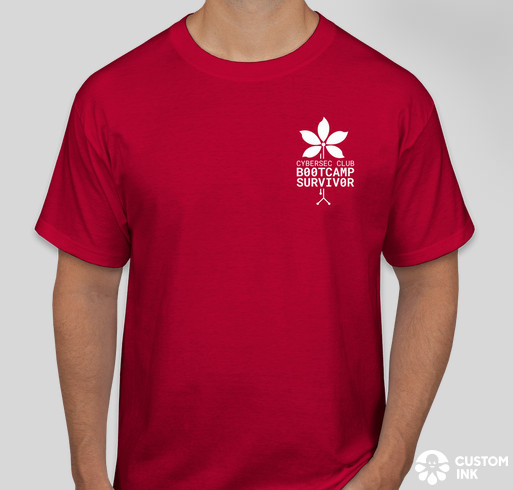
\includegraphics[width=0.3\paperwidth]{shirt1.png}};
        \node[left = of shirt1] (shirt2) {
\includegraphics[width=0.3\paperwidth]{shirt2.png}};
        \node[anchor=north east, yshift=-4cm, xshift=-2cm] (sticker) at (current page.north east) {
\includegraphics[width=0.3\paperwidth]{sticker.png}};
    \end{tikzpicture}
\end{frame}

\setbeamercolor{background canvas}{bg=almostblack}
\setbeamertemplate{section in toc}[square]
\begin{frame}
    \frametitle{Overview} % Table of contents slide, comment this block out to remove it
    \tableofcontents % Throughout your presentation, if you choose to use \section{} and \subsection{} commands, these will automatically be printed on this slide as an overview of your presentation
\end{frame}

\section{What is reverse engineering?}
\begin{frame}
    \frametitle{What is reverse engineering?}
    \begin{itemize}
        \item{\textbf{"...the process by which a man-made object is deconstructed to reveal its designs, architecture, code, or to extract knowledge from the object"}}
        \item{tl;dr Figure out how something works}
        \begin{itemize}
            \item{Often with limited or no documentation}
            \item{With a required level of understanding that varies depending on the task}
        \end{itemize}
        \item{Examples}
        \begin{itemize}
            \item{Figure out how a co-workers code works after they got fired}
            \item{Figure out how a game communicates in a multiplayer session... for 'research' of course}
            \item{Figure out how a streaming service plays audio/video... (note: piracy bad)}
        \end{itemize}
    \end{itemize}
\end{frame}

\subsection{About Computers}
\begin{frame}
    \frametitle{About computers}
    \framesubtitle{CSE 3421 in 3 minutes}
    \begin{itemize}
        \item{A computer understands a defined set of 'instructions', which each perform some small operation (arithmetic, data movement, I/O, control flow)}
        \begin{itemize}
            \item{x86 vs. ARM vs. [...]}
        \end{itemize}
        \item{Programmers should assume instructions run \textbf{'serially'} (one at a time, in sequence)}
        \item{Programs can interact with memory as a 'sea of byte-addressable bits'}
    \end{itemize}
    \begin{bytefield}[bitwidth = 1.5em, leftcurly = .]{16}
        \bitheader[endianness = little]{0-15}\\
        \bytefieldsetup{}%
        \begin{leftwordgroup}{Memory}
		\bitboxes*{1}{{47} {6F} {20} {42} {75} {63} {6B} {72} {00} {00} {00} {00} {00} {00} {00} {00} }
        \end{leftwordgroup}\\[1ex]
    \end{bytefield}
\end{frame}


\begin{frame}
    \frametitle{About computers}
    \framesubtitle{CSE 3421 in 3 minutes}
    \begin{itemize}
	\item{"Get me 8 bytes at address 0x42, store it in register 1"}
        \item{"Add register 1 to register 2, put the result in register 1"}
        \item{"Get me 8 bytes using address in register 1, put the result in register 1}
        \item{"Move the data from register 1 into register 2"}
	\item{"If the value in register 1 is nonzero, jump to code at address 0x1337"} 
    \end{itemize}
    \begin{bytefield}[bitwidth = 1.5em, leftcurly = .]{16}
        \bitheader[endianness = little]{0-15}\\
        \bytefieldsetup{}%
        \begin{leftwordgroup}{Memory}
		\bitboxes*{1}{{47} {6F} {20} {42} {75} {63} {6B} {72} {00} {00} {00} {00} {00} {00} {00} {00} }
        \end{leftwordgroup}\\[1ex]
    \end{bytefield}
\end{frame}

\begin{frame}
    \frametitle{Machine code is everything}
    \framesubtitle{or, everything is machine code}
    \begin{itemize}
	    \item{\textbf{Native applications (compiled code):} Compile to machine code, distribute to users, then they run it}
        \item{\textbf{JIT-ed languages:} You write Javascript, the browser 'just-in-time' translates your Javascript into machine code, and then runs it.}
	\item{\textbf{Interpreted languages:} An interpreter directly runs the source code, line by line, implementing all the behaviors of the language. e.g. CPython (the most common Python implementation)}
	\item{\textbf{Often, a combination of the above...} The line is blurry.}
    \end{itemize}

\end{frame}

\begin{frame}
    \begin{tikzpicture}[overlay]
        \node[anchor=south east, yshift=-5cm, xshift=-4cm] (shirt1) at (current page.south east) {
\includegraphics[width=0.5\paperwidth]{turtle.png}};
    \end{tikzpicture}

\end{frame}

\section{Useful Tools and What They Do}
\begin{frame}
    \frametitle{Tools}
    \begin{itemize}
        \item{tbd}
    \end{itemize}
\end{frame}


\begin{frame}
    \frametitle{Recommended Challenges}
    \begin{itemize}
        \item{Also, any challenge 25 pt or less should be solvable before we talk about that category}
    \end{itemize}
\end{frame}

\begin{frame}
    \frametitle{Possible Future Topics}
    \begin{itemize}
	\item{\textbf{topics}}
    \end{itemize}
\end{frame}

\end{document}
